\documentclass[12pt]{article}

\usepackage[margin=1.9cm, letterpaper]{geometry}
\usepackage[utf8]{inputenc}
\usepackage{listings}
\usepackage{xcolor}
\usepackage{graphicx}
\usepackage{indentfirst}
\usepackage{tikz}
\usepackage{float}
\usepackage{fancyvrb}
\usepackage{subcaption}
\usepackage{pdfpages}
\usepackage{amsmath}
\usepackage{amssymb}

\usepackage{subfiles}

\usepackage{parskip}
\setlength{\parskip}{1em}
\setlength{\parindent}{2em}

\usetikzlibrary{shapes.geometric, arrows}

\renewcommand{\thesection}{}
\renewcommand{\thesubsection}{}

\lstdefinestyle{mystyle}{
    basicstyle=\ttfamily\footnotesize,
    tabsize=4
}


\begin{document}
\begin{titlepage}
    \begin{center}
    \vspace*{1cm}
    
    \textbf{Lab 3}

    \vspace{0.5cm}

     Subroutines
    
    \vspace{1.5cm}

    \textbf{Hans Jarales (1537516) and Michael Kwok (1548454)}

    \vfill
            
    ECE 212 Lab - Introduction to Microprocessors\\
    Department of Electrical and Computer Engineering\\
    University of Alberta\\
    April 1, 2020    

   \end{center}
\end{titlepage}

\tableofcontents
\pagebreak

\section{Introduction}
In this lab, we implement a program on the ColdFire development board to calculate certain statistics about a set of numbers given through input by a user.
Subroutines were utilized and explored in the implementation of this program. Three main subroutines were used respectively in prompting the user for the data, analyzing the data, calculate statistics, and then returning the results to the user. All the subroutines are transparent, meaning all registers were backed up then restored afterwards. Provided are supplementary subroutines/functions to aid in displaying certain strings to the user, and displaying data. Further explored was the use and operation of the stack and the corresponding stack pointer. Special attention was required in keeping track of the contents of the stack and the stack pointer -- negligence towards the stack's contents can result in improper use of the subroutines/functions that depend on it.


\section{Design}
\subsection{Part A}
The subroutine designed and implemented in Part A is to solely prompt the user for data to be analyzed via input.

A series of string messages are associated with every prompt, stored in the \textbf{.data} section of this subroutine. These strings were displayed using the \textbf{iprintf} function which worked under the condition that the string address was located on the stack. The string address is then pushed onto the stack before the function is called. After the function is called and the string gets displayed, the string address remains on the stack, and should be removed before continuing.

\begin{verbatim}
Listing 1.
    pea     <string label from .data>   /*Push address onto stack*/
    jsr     iprintf                     /*Display string*/
    adda.l  #4, %sp                     /*Remove string address -- restore sp*/
    jsr     cr                          /*Create new line*/
    ...
\end{verbatim}

The \textbf{getstring} function is used to take in user input and store it into register \textbf{d0}. The subroutine is to make sure the numbers entered are within the acceptable range. The number of entries is first determined, with an acceptable range of 3-15 entries. Second, the divisor is determined, which can be a number between 2 and 5. Finally, the set of numbers is gathered from the user, where all the entries must be positive. The number of entries, and the divisor number are then stored in predetermined locations on the stack to be used for analyses by later subroutines. The entries are stored at an array starting at location 0x43000000.

\begin{verbatim}
Listing 2.
    PromptMsg:
        /*Display string message*/
        /*Take input*/
        bra InputCheck
    InvalidInput:
        /*Display string message*/
        /*Take input*/
    InputCheck:
        /*Check if input is within acceptable conditions*/
        /*If invalid, branch to InvalidInput*/
        /*Otherwise, store result onto corresponding location on stack*/
    ...
\end{verbatim}

The available data and address registers are backed up and restored in this subroutine through the use of the stack and the stack pointer (\textbf{sp} or \textbf{a7}). To store the input data to the required locations on the stack, the backed up registers, the called functions, and therefore the stack pointer needed to be kept track of. The stack pointer needed to be offset by the correct index such that the data input is to be stored in the correct position. Before the Part A subroutine is called by the main program, the stack pointer points towards where the divisor number should be stored, followed by where the number of entries should be stored, where both are longword-sized. After the Part A subroutine is called, the stack pointer then is positioned on the return address. Then, the registers are backed up. Where there were in total 10 registers backed up, the stack pointer is then decremented by 40 bytes from its previous position to store the registers' contents on the stack.  In this, the stack pointer with an offset of 44 is used to store the divisor number collected from the user. Similarly, an offset of 48 is used on the stack pointer to store the number of entries.
\begin{center}
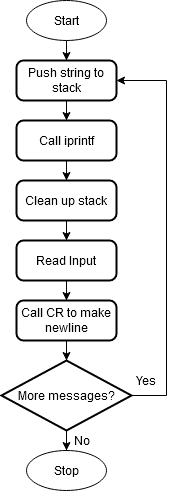
\includegraphics[scale = 0.5]{./PartA.PNG}
\end{center}
\subsection{Part B}
The Part B subroutine is to calculate certain statistics of the given numbers. The mean is calculated from the given numbers. The maximum and minimum of the numbers is also found. Finally, the number of entries and the entries themselves that are divisible by the divisor number collected earlier is produced. 

The search for the largest (maximum) and the smallest (minimum) number among the input entries follow the same process. The design for finding the minimum is shown:

\begin{verbatim}
Figure[3] 
    FindMin:
        /*Utilize information from the stack provided by the Part A Subroutine*/
        move (%a2)+,  d2    /*a2 points to the array of entries*/
        move 48(%sp), d4    /*make counter with number of entries*/
    MinLoop:
        /*Decrement counter (d4)*/
        /*If counter (d4) is zero, exit loop onto next analysis*/
        /*Test the array of numbers to find the minimum number*/
        move (%a2)+,  d3
        /*Compare d3 to d2*/
        /*If d3 > d2, d2 remains the minimum, and the loop is restarted/
        /*Otherwise, d3 is stored into d2, and the loop is restarted*/
    
    /* Store minimum into array containing results pointed by a3*/
    move d2, (%a3)+
    ...
\end{verbatim}

Calculating the mean involves adding up the entries entered by the user, and dividing this sum by the number of entries. The subroutine achieves this through use of a loop to accumulate a sum of the entries. When all the entries are are summed, they are divided by the number of entries found at the bottom of the stack.

\begin{verbatim}
Figure[4]
    FindMean:
        /*Renitialize address to array of entries*/
        /*Reload counter*/
        /*Clear d2 to use as an accumulated sum of entries*/
    MeanLoop:
        /*Add entries to d2*/
        /*Decrement counter -- restart MeanLoop if not 0*/
        /*Divide d2 by number of entries located at 48(%sp)*/
        /*Move d2 to output array pointed by a3*/
\end{verbatim}

Each number from the data array is tested with the divisor number. This is done with a loop conditioned on the number of entries. Each data entry is divided by the divisor number using \textbf{divu.w}: this returns a longword-sized result containing both the quotient in the lower word and the remainder in the higher word of the longword result:

\begin{verbatim}
Figure[5]
    /*Let d0 = 0x21, d1 = 0x10*/
    divu.w %d1, %d0 /*Divide 0x21 by 0x10*/
    
    /*Result: Quotient = 2 Remainder = 1*/
    /*d0 now contains: 0x 0001 0002*/
\end{verbatim}

In checking if the data entry is indeed divisible, the remainder is tested. If there is no remainder, the data entry is indeed divisible -- the counter tracking the number of divisible entries is incremented and the data entry itself is stored into the output array pointed by a3. Otherwise, the loop is reset and the next data entry is tested.

\begin{verbatim}
Figure[6]
    FindDivisible:
        /*Move data entry into d2*/
        /*Copy data entry from d2 into d4 for analysis*/
        /*Get divisor number from bottom of stack located 44(%sp)*/
        divu.w %d7, %d4/*Divide d4 with divisor number in d7*/
    
    remaindercheck:
        /*Isolate remainder: */
        and.l #0xFFFF0000, %d4
        /*If the remainder is zero, move d2 into the output array and
        increment the divisor counter d6*/
        /*Otherwise, decrement the counter of entries and restart loop*/
\end{verbatim}

The number of divisible data entries is moved onto the bottom of the stack, located now at \textbf{52(sp)}. Again, the registers are initially backed up, and restored.

\begin{center}
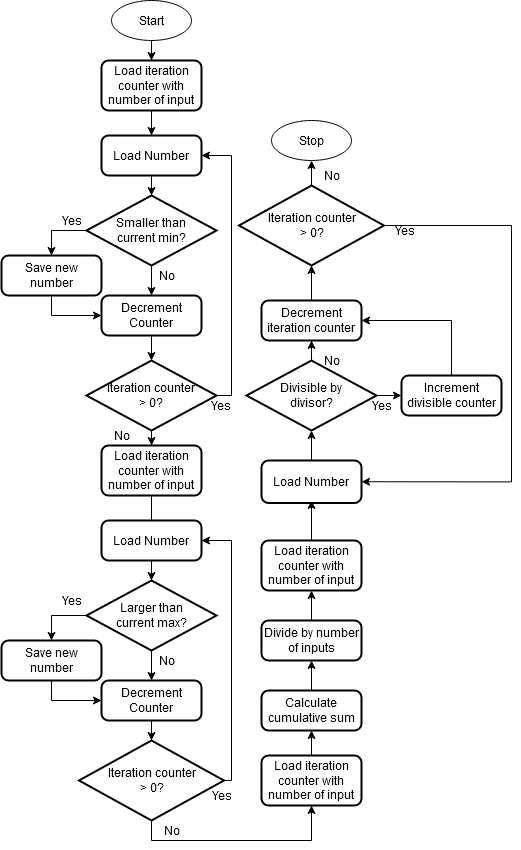
\includegraphics[scale = 0.5]{./PartB.PNG}
\end{center}

\subsection{Part C}
The Part C subroutine takes the results of the statistics collected and prints them out to the user. 

In this subroutine, new string messages are made in the \textbf{.data} section to display using \textbf{iprintf} and \textbf{cr}, along with the data and calculations. Displaying the numbers is done using the \textbf{value} function. This function requires the desired number to be on top of the stack. The process behind printing the divisor number is shown:

\begin{verbatim}
Figure[7]
    move.l 44(%sp), d2 /*Move divisor number to d2*/
    move.l d2, -(%sp)  /*Move divisor number on top of stack*/
                       /*sp is decremented since it points to the
                       return address after this subroutine is called*/
    jsr value           /*Print divisor number*/
    adda.l #4, %sp      /*Remove divisor number from stack*/
    jsr cr              /*Create newline*/
   ...
\end{verbatim}

A similar process is used to display the rest of the relevant numbers.

\begin{center}
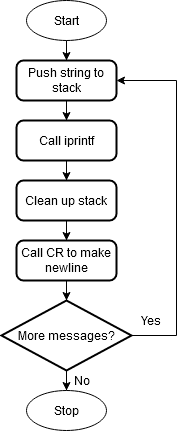
\includegraphics[scale = 0.5]{./PartC.PNG}
\end{center}

\section{Questions}
\begin{enumerate}
    \item Is it always necessary to implement either callee or caller preservation of registers when calling a subroutine. Why?
    \begin{itemize}
        \item It is necessary to implement one or the other as registers are a shared resource. Many assembly commands do not work directly on the memory, and require usage of the register. If neither the callee nor the caller preserves the registers, data might get lost from either one.
    \end{itemize}
    \item Is it always necessary to clean up the stack. Why?
    \begin{itemize}
        \item Not removing unnecessary content on the stack results in an incorrect stack pointer; incorrect data can be used from the stack, and in some cases, performing \textbf{rts} at the end of the subroutine whilst the stack pointer is not positioned at the return address results in an error or incorrect instruction executed afterwards, as \textbf{rts} might take a piece of data instead of an address and attempt to jump there.
    \end{itemize}
    \item If a proper check for the getstring function was not provided and you have access to the buffer, how would you check to see if a valid \# was entered?  A detailed description is sufficient. You do not need to implement this in your code.
    \begin{itemize}
        \item A simple check for valid numbers would be to compare the ASCII code of the input. If it was between \Verb#0x30# and \Verb#0x39# inclusive, it is a valid number. The check can be repeated for the entire string up to the \Verb#0x0# character is read. The check can be implemented by reading the string, running the comparison, converting ASCII to BCD, storing it into a register. The register would get multiplied by 10 then the same actions starting from the check will be repeated for the next character until the null-terminator or a non-numeric character gets read.
    \end{itemize}
\end{enumerate}

\section{Conclusions}
This lab focuses mainly on the usefulness behind the successful execution of subroutines, and the purposes of the stack. The subroutines when used in concert make for programs that are easier to implement, and are generally more organized and less difficult to understand. This was most notably seen in the use of the provided supplementary functions (\textbf{iprintf, cr, value, and getstring}). These functions were used repetitively throughout the first and last subroutines. These functions highlight the efficiency and easy implementation behind creating functions in place of repetitive operations in a program.

Also highlighted, is the importance in cleaning up, and keeping track of the stack contents and stack pointer throughout the design of the subroutines.
\pagebreak

\section{Appendix}
\renewcommand{\thepage}{}
\subsection{Part A Assembler Code}
\lstinputlisting[language={[Motorola68k]Assembler}, style={mystyle}]{Lab3/Lab3a.s}
\pagebreak
\subsection{Part B Assembler Code}
\lstinputlisting[language={[Motorola68k]Assembler}, style={mystyle}]{Lab3/Lab3b.s}
\subsection{Part C Assembler Code}
\lstinputlisting[language={[Motorola68k]Assembler}, style={mystyle}]{Lab3/Lab3c.s}


\includepdf[pages=-]{lab3markingsheet.pdf}

\end{document}